\chapter{Perbaikan Citra}
\section{Pendahuluan}

Perbaikan citra dilakukan dengan cara menghilangkan/mengurangi degradasi citra yang dapat disebabkan karena \textit{noise} atau \textit{blurring}. Degradasi sebuah citra digital dapat dimodelkan dengan persamaan (\ref{eq:degradeModel})\cite{Gonzalez}.

\begin{equation}
g(x,y)=\left(f(x,y)*h(x,y)\right)+n(x,y)
\label{eq:degradeModel}
\end{equation}
 
 Dari persamaan (\ref{eq:degradeModel}), diketahui
 \begin{itemize}
   \item $g(x,y)$ adalah citra terdegradasi
   \item $f(x,y)$ adalah citra asli
   \item $h(x,y)$ adalah filter spasial
   \item $n(x,y)$ adalah \textit{noise}
 \end{itemize}
 Dengan demikian, secara teoritis, citra asli dapat kembali diperoleh dengan menggunakan persamaan (\ref{eq:restore}). Tentu dengan mengetahui fungsi \textit{noise} yang menyebabkan citra terdegradasi.
 
 \begin{equation}
   f(x,y)=\frac{g(x,y)-n(x,y)}{h(x,y)}
   \label{eq:restore}
 \end{equation}
 
 \section{\texttt{random\_noise}}
 Pustaka \texttt{scikit-image} menyediakan fungsi degradasi citra dengan nama \texttt{random\_noise} yang diletakkan di bawah sub modul \texttt{util}. Fungsi tersebut memfasilitasi pemberian beberapa jenis \textit{noise} berikut karakteristiknya masing-masing. Berikut adalah beberapa contoh pemberian \textit{noise}. 
 
 Fungsi \texttt{random\_noise} menerima argumen berikut ini.
 \begin{enumerate}
   \item \texttt{image} adalah citra yang akan diberi \textit{noise}, fungsi akan secara otomatis melakukan normalisasi nilai intensitas citra pada rentang \texttt{0} s/d \texttt{1}.
   \item \texttt{mode} adalah jenis \textit{noise} yang dapat diberikan dalam tipe data \texttt{str}. Jenis \textit{noise} tersebut adalah
   \begin{itemize}
     \item 'gaussian' tambahan \textit{noise} yang memenuhi distribusi Gaussian
     \item 'localvar' tambahan \textit{noise} yang memenuhi distribusi Gaussian dengan tambahan informasi \textit{local variance} pada setiap titik citra. Jika argumen \texttt{mode} bernilai 'localvar', argumen \texttt{local\_vars} harus diberikan 
     \item 'poisson' tambahan \textit{noise} yang memenuhi distribusi Poisson
     \item 'salt' tambahan \textit{noise} yang mengubah titik piksel yang dipilih secara acak dengan nilai \texttt{1}
     \item 'pepper' tambahan \textit{noise} yang merupakan kebalikan dari 'salt'. \textit{Noise} 'pepper' mengubah titik piksel yang dipilih secara acak dengan nilai \texttt{1} (untuk jenis \textit{unsigned}) atau \texttt{-1} (untuk jenis \textit{signed})
     \item 's\&p' adalah tambahan \textit{noise} yang merupakan gabungan jenis 'salt' dan 'pepper'
     \item 'speckle' adalah tambahan \textit{noise} yang mengubah nilai intensitas citra pada setiap piksel menjadi $x+(n*x)$, dengan $x$ adalah intensitas citra asli dan $n$ adalah fungsi \textit{uniform noise} dengan tambahan argumen \texttt{mean} (rerata) dan \texttt{var} (varians) 
   \end{itemize}
   \item \texttt{seed} bertipe \texttt{int} dan bersifat opsional. Tetapi, jika nilai argumen diberikan, nilai tersebut akan digunakan untuk menghasilkan nilai acak untuk membangkitkan \textit{noise}
   \item \texttt{clip} bertipe \text{bool} dan bersifat opsional. Jika tidak diberikan, maka fungsi \texttt{random\_noise} akan memberikan nilai \texttt{True} pada argumen ini. Dampaknya, hasil pemberian \textit{noise} dari jenis 'speckle', 'poisson' dan 'gaussian' membuat citra tetap memiliki rentang nilai intensitas [-1,1] (\textit{unsigned}). Sebaliknya, jika secara aktif diberikan nilai \texttt{False}, citra hasil pemberian \textit{noise} dapat memiliki nilai intensitas di luar rentang normalnya
   \item \texttt{mean} adalah nilai rerata dari distribusi \textit{noise} 'gaussian' dan 'speckle'. Argumen ini bertipe \texttt{float} dan bersifat opsional. Jika tidak diberikan, fungsi \texttt{random\_noise} akan memberikan nilai \texttt{0} untuk argumen ini.
   \item \texttt{var} adalah nilai varians untuk distribusi \textit{noise} 'gaussian' dan 'speckle'. Argumen ini menerima nilai \texttt{float} dan bersifat opsional. Jika tidak diberikan, fungsi \texttt{random\_noise} akan memberikan nilai \texttt{0.01}
   \item \texttt{local\_vars} adalah argumen yang diperlukan ketike pengguna memberikan \textit{noise} dengan \texttt{mode} 'localvar'
   \item \texttt{amount} adalah argumen yang digunakan untuk menentukan proporsi jumlah piksel yang akan dikonversi nilai internsitasnya ketika \texttt{mode} 'salt', 'pepper' dan 's\&p' digunakan.
   \item \texttt{salt\_vs\_pepper} adalah argumen yang digunakan untuk menentukan proporsi jumlah piksel yang nilai intensitasnya akan dikonversi menjadi \texttt{1} ('salt') dan \texttt{0}/\texttt{-1} ('pepper'). Argumen ini diberikan ketika \texttt{mode} bernilai 's\&p'
 \end{enumerate}
 
\figurename~\ref{fig:addNoise} menunjukkan perbandingan citra asli dan citra dengan penambahan \textit{noise} dari fungsi Gaussian.
 
\begin{figure}[h!]
\begin{center}
\subfigure[]{\label{fig:asli}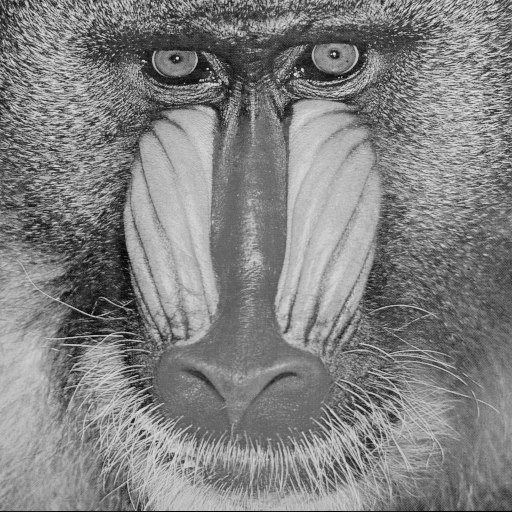
\includegraphics[scale=.35]{pics/baboonGS.png}}
\subfigure[]{\label{fig:nois}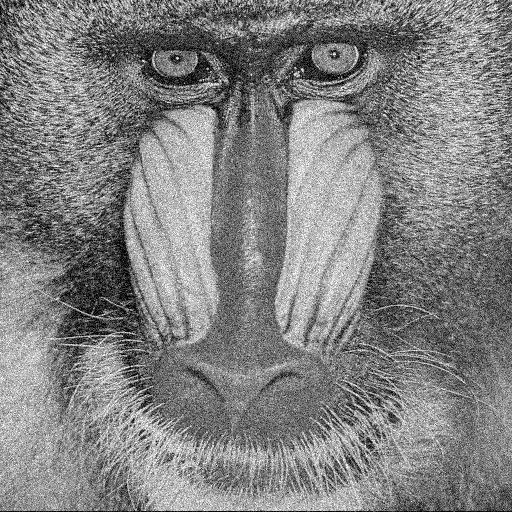
\includegraphics[scale=.35]{pics/baboonNoise.png}}
\caption{Perbandingan (a). citra asli, (b). citra dengan penambahan \textit{noise} Gaussian dengan nilai \texttt{mean=0} dan \texttt{var=0.01}}
\label{fig:addNoise}
\end{center}
\end{figure}

\section{\textit{Spatial denoizing}}
Pustaka \textit{scikit-image} menyediakan fungsi pengurangan \textit{noise} secara spasial pada sub modul \texttt{skimage.filters.rank}. Sub bab ini akan menunjukkan hasil dari pengurangan \textit{noise} secara spasial berbasis sejumlah opsi \textit{structuring element} (dibahas di bab \ref{sec:morph}). 

\lstlistingname~\ref{lst:denoise} menjelaskan proses pengurangan \textit{noise} dengan filter \texttt{mean} dan \textit{structuring element} berupa matriks segiempat dengan nilai elemen penyusunnya yang membentuk segiempat (\texttt{square}) dan lingkaran (\texttt{disk}). Sedangkan \figurename~\ref{fig:deNoise} menunjukkan perbedaan hasil pengurangan \textit{noise} terhadap \figurename~\ref{fig:nois}.

\scriptsize
\lstinputlisting[language=python, numbers=left, numberstyle=\tiny, caption=Pengurangan \textit{noise} dengan filter spasial, showstringspaces=false, label=lst:denoise]{script/denoise.py}
\normalsize

\begin{figure}[h!]
\begin{center}
\subfigure[]{\label{fig:sq3}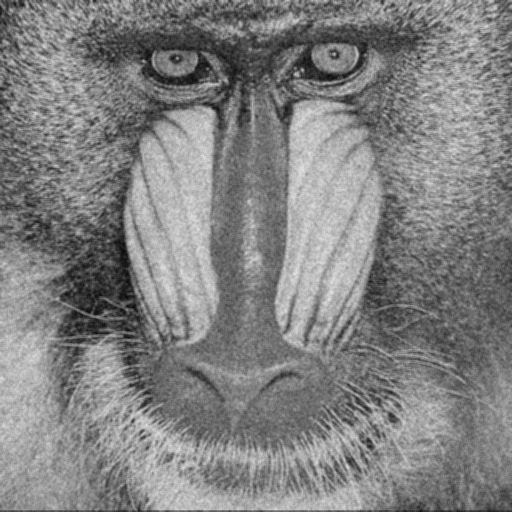
\includegraphics[scale=.35]{pics/baboonSquare3.png}}
\subfigure[]{\label{fig:sq5}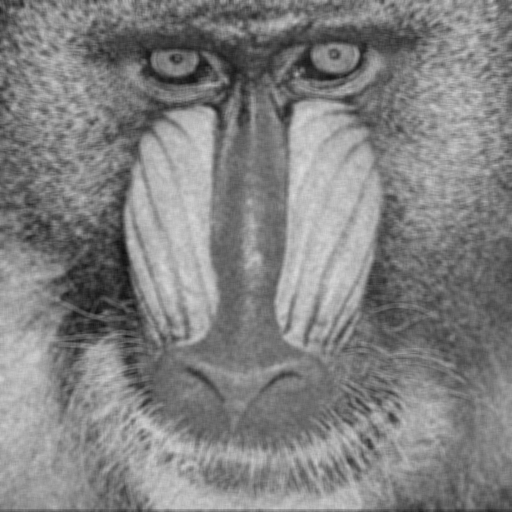
\includegraphics[scale=.35]{pics/baboonSquare5.png}}
\subfigure[]{\label{fig:disk1}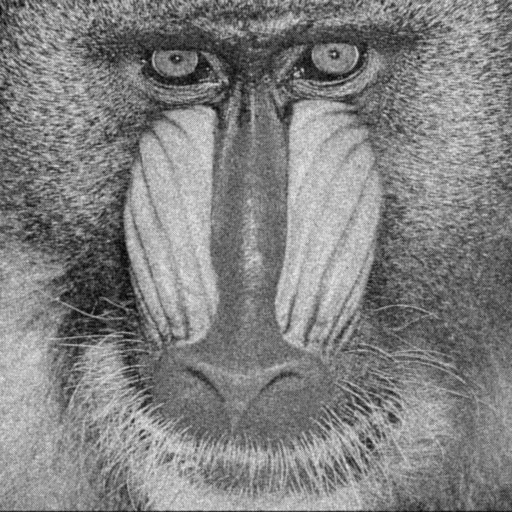
\includegraphics[scale=.35]{pics/baboonDisk1.png}}
\subfigure[]{\label{fig:disk2}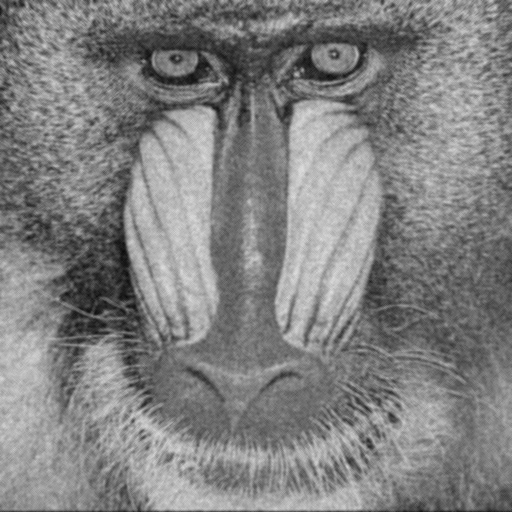
\includegraphics[scale=.35]{pics/baboonDisk2.png}}
\caption{Hasil pengurangan \textit{noise} dengan \textit{structuring element} (a). \texttt{square(3)}, (b). \texttt{square(5)}, (c). \texttt{disk(1)} dan (d). \texttt{disk(2)}}
\label{fig:deNoise}
\end{center}
\end{figure}

\section{\textit{Frequency domain denoizing}}
\label{sec:freqDenoizing}
Setiap fungsi yang berulang secara periodik dapat dinyatakan sebagai jumlah dari beberapa fungsi pada frekuensi dan amplitudo tertentu \cite{Gonzalez}. Ilustrasinya disajikan pada \figurename~\ref{fig:periodik}. Sebuah citra digital dapat dianggap sebagai fungsi periodik yang karenanya dapat ditransformasi ke dalam domain frekuensi. Pada posisi di mana terjadi perubahan nilai intensitas piksel secara signifikan, citra dikatakan menyimpan komponen frekuensi tinggi. Sebaliknya, pada posisi di mana perubahan intensitas piksel sangat landai bahkan nyaris tetap, citra dikatakan menyimpan komponen frekuensi rendah.

\begin{figure}
  \begin{center}
    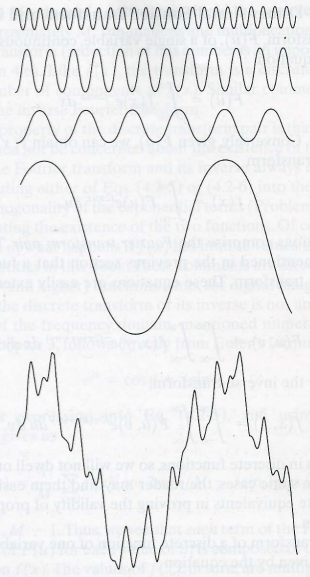
\includegraphics[scale=.5]{pics/fourierBasic.png}
    \caption{Fungsi periodik yang merupakan kombinasi dari beberapa fungsi periodik lain}
    \label{fig:periodik}
  \end{center}
\end{figure}

Pada frekuensi tinggi, di situlah batas obyek umumnya berada. Mempertahankan komponen frekuensi tinggi akan menjaga kontras citra tetap baik. Sebaliknya, frekuensi rendah merepresentasikan kondisi di mana nilai intensitas piksel cenderung tetap. Mempertahankan komponen frekuensi rendah menjadi dasar dari proses penghalusan (\textit{smooting}) citra.

Secara teori, mempertahankan/menghilangkan komponen dengan frekuensi/rentang frekuensi tertentu dari citra dilakukan pada domain frekuensi. Citra harus ditransformasi dahulu ke domain frekuensi. Selanjutnya, komponen frekuensi yang tidak diharapkan dapat dihilangkan. Terakhir, transformasi dilakukan kembali ke domain spasial. Dengan pustaka \texttt{scikit-image}, proses transformasi dilakukan secara implisit oleh fungsi \texttt{difference\_of\_gaussian} di bawah sub modul \texttt{filters}. Fungsi tersebut sejatinya adalah sebuah \textit{band pass filter}, filter untuk menyaring rentang frekuensi tertentu. Frekuensi dinyatakan sebagai nilai $\sigma$ (standar deviasi). Ilustrasinya disajikan pada \figurename~\ref{fig:gaussian}.

\begin{figure}
  \begin{center}
    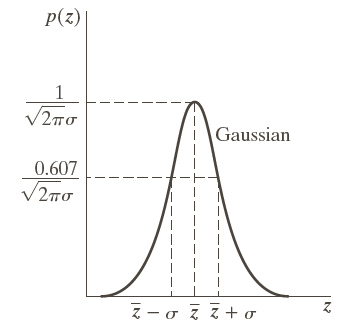
\includegraphics[scale=.6]{pics/gaussian.png}
    \caption{Ilustrasi kurva dengan fungsi gaussian}
    \label{fig:gaussian}
  \end{center}
\end{figure}

Semakin besar nilai $\sigma$ maka frekuensi semakin kecil. Sebaliknya, semakin kecil nilai $\sigma$, maka frekuensi semakain besar. Ilustrasinya disajikan pada \figurename~\ref{fig:sigmaFrekuensi}. Nilai $\sigma$ di \figurename~\ref{fig:cth1} lebih besar dibandingkan di \figurename~\ref{fig:cth2}. Besarnya nilai $\sigma$ ditunjukkan dengan bentuk kurva yang melebar dan dengan amplitudo kecil (\figurename~\ref{fig:cth1}). Sedangkan besarnya nilai frekuensi ditunjukkan dengan bentuk kurva yang pipih dengan amplitudo besar (\figurename~\ref{fig:cth2}).

\begin{figure}
\begin{center}
\subfigure[]{\label{fig:cth1}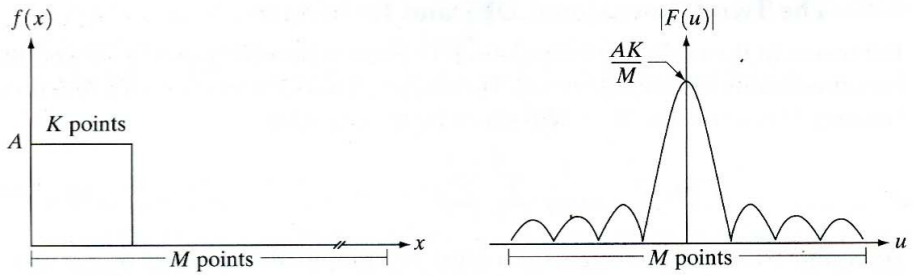
\includegraphics[scale=.35]{pics/contoh1.png}}
\subfigure[]{\label{fig:cth2}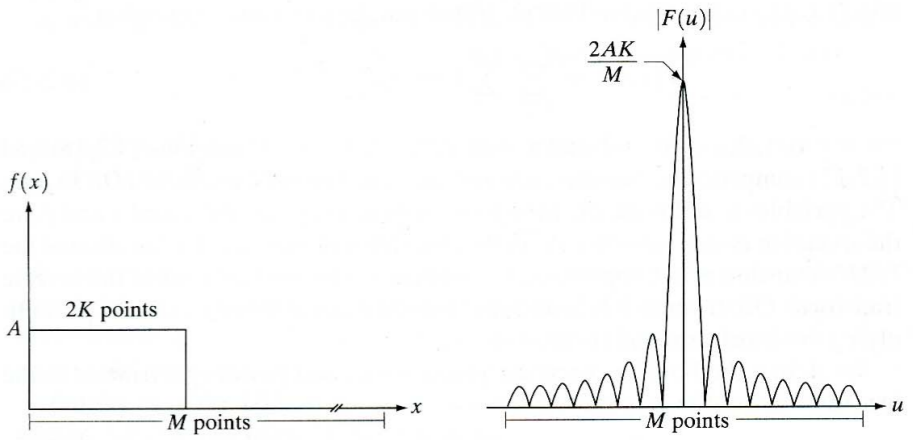
\includegraphics[scale=.35]{pics/contoh2.png}}
\caption{Ilustrasi perbandingan nilai $\sigma$ terhadap frekuensi}
\label{fig:sigmaFrekuensi}
\end{center}
\end{figure}

Sedangkan \figurename~\ref{fig:filteringFreq} menunjukkan hasil penyaringan frekuensi rendah, sedang (pada rentang frekuensi tertentu), dan tinggi dari citra baboon dalam warna RGB. Penyaringan tersebut dilakukan dengan fungsi \texttt{difference\_of\_gaussian}. \figurename~\ref{fig:highPass} diperoleh dengan memberikan argumen \texttt{low\_sigma=0} dan \texttt{high\_sigma=5}. Pemberian argumen dengan nilai tersebut bermakna frekuensi tertinggi yang ada di dalam citra hingga frekuensi yang setara dengan nilai $\sigma=5$ akan dipertahankan. Terlihat bahwa \figurename~\ref{fig:highPass} terlihat lebih jelas daripada kedua citra lainnya.

Selanjutnya, pembentukan citra pada \figurename~\ref{fig:bandPass}, argumen yang diberikan untuk \texttt{low\_sigma=5} dan \texttt{high\_sigma=10}. Pemberian argumen tersebut akan menyaring frekuensi yang setara dengan nilai $\sigma=10$ hingga frekuensi yang setara dengan nilai $\sigma=5$ akan dipertahankan. Karena frekuensi yang setara dengan nilai $\sigma=5$ atau lebih dihilangkan, maka citra di \figurename~\ref{fig:bandPass} terlihat semakin buram jika dibandingkan dengan citra pada \figurename~\ref{fig:highPass}.

Terakhir, pembentukan citra pada \figurename~\ref{fig:LowPass}, argumen yang diberikan untuk \texttt{low\_sigma=10} sedangkan argumen \texttt{high\_sigma} tidak diberikan. Dengan kombinasi tersebut, frekuensi yang setara dengan nilai $\sigma=10$ dan yang lebih rendah akan dipertahankan. Berarti yang tersisa dari citra adalah komponen frekuensi rendah. Hasilnya, \figurename~\ref{fig:LowPass} tampak paling buram dibanding dua citra sebelumnya.

\begin{figure}
\begin{center}
\subfigure[]{\label{fig:highPass}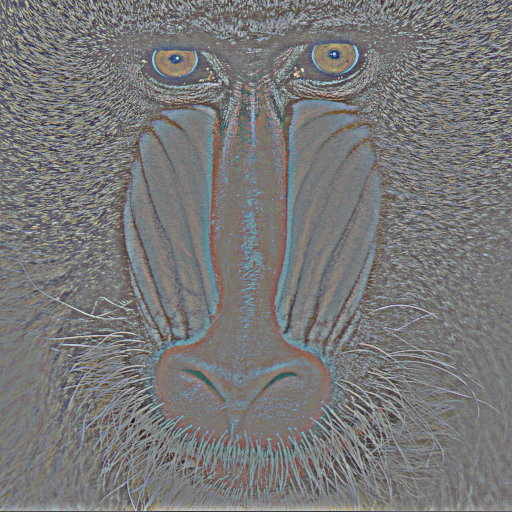
\includegraphics[scale=.25]{pics/baboonFiltered05.png}}
\subfigure[]{\label{fig:bandPass}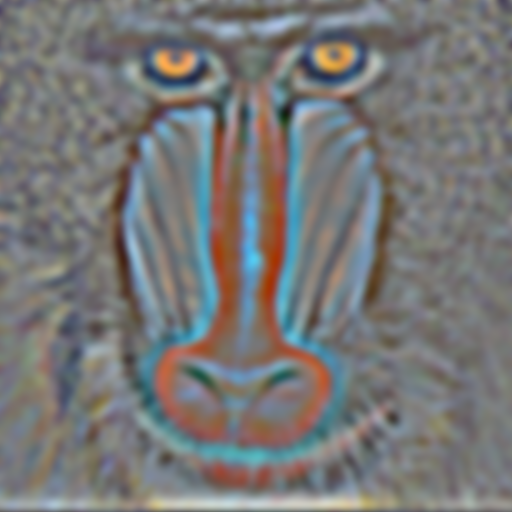
\includegraphics[scale=.25]{pics/baboonFiltered.png}}
\subfigure[]{\label{fig:LowPass}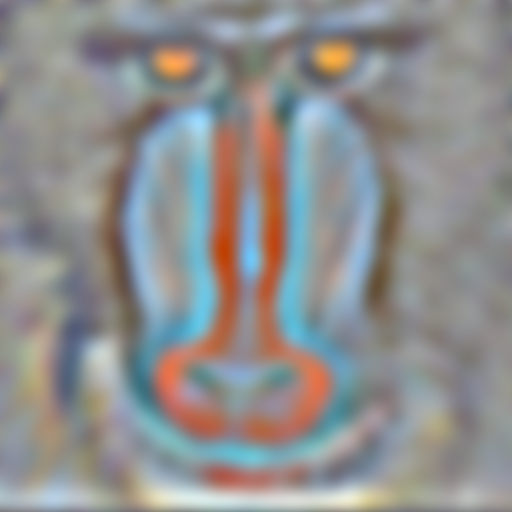
\includegraphics[scale=.25]{pics/baboonFiltered10.png}}
\caption{Hasil penyaringan frekuensi rendah, sedang dan tinggi pada citra RGB}
\label{fig:filteringFreq}
\end{center}
\end{figure}
